\documentclass[a4paper,14pt]{report}
\usepackage[utf8]{inputenc}
\usepackage{layout}
\usepackage[top=2cm, bottom=2cm, left=3cm, right=2cm]{geometry}
\usepackage{setspace}
\usepackage{plain}
\usepackage{mathtools, bm}
\usepackage{amssymb, bm}
\usepackage{geometry}
\geometry{hmargin=2.5cm,vmargin=2.5cm}

\title{Conclusion Focus Groupe}
\author{PACT 3.5}
\begin{document}
\maketitle




\begin{center}
\textbf{Description du dispositif}
\end{center}

Ce focus groupe avait pour support 6 extraits de textes de Harry Potter. 3 extraits portaient sur le thème 
de noël : lorsque Harry ouvre ses cadeaux de noël et les 3 autres sur le thème Quidditch : lors des matchs de 
Quidditch. \\
Une personne interrogée avait le choix entre un des deux thèmes. Lorsque celui-ci est choisi, elle lisa 3 extraits. Le premier extrait se fait avec une odeur et une ambiance imposée (qui est selon nous adaptée à l'extrait). Le deuxième extrait se lit de manière personnalisée : le testeur a le choix entre une gamme d'ambiance sonore (une dizaine) et d'odeur (entre 5 et 6). Enfin, le troisième et dernier extrait se fait sans odeur ni ambiance sonore.
L'expérience se présentait de la manière suivante : nous demandions à la personne interrogée de s'installer au fond d'une salle (généralement la C49 ou C47) sur une chaise. Nous lui expliquions le principe de l'expérience et lui demandions de choisir une odeur pour le deuxième extrait. Nous avions une tablette avec l'application dessus et généralement un casque pour les sons. Généralement, une personne du groupe supervisait les odeurs et une autre la gestion de la tablette et des questions d'après expérience. \\
Lors de la fin de l'expérience (la lecture des trois extraits), nous invitions la personne à répondre à 5 questions qualitatives sur ce qu'ils ont pensé des 3 expériences. Ensuite, une semaine après l'expérience, un autre questionnaire d'une dizaine de question leur était envoyé. Ce second questionnaire comportait des questions sur leurs ressenties de l'expérience et des questions très précises sur le texte afin de voir les effets de la stimulation de plusieurs sens sur la mémoire. Il y avait entre 2 à 3 questions sur chaque texte. Les extraits sur le thème de noël étaient notées sur 30 points (10 points par texte) et le 15 points pour le thème Quidditch (5 points par texte). Nous avions préparé les réponses aux questions afin de pouvoir les corriger rapidement.\\
Des photos du dispositif sont disponibles en fin de document. 




\begin{center}
\textbf{Personnes interrogées} 
\end{center}

Nous avons réalisé cette expérience sur 10 personnes. Ces dernières sont des élèves de l'école (Télécom Paristech) : en effet, l'expérience se réalisait à l'intérieur des locaux. Seule une personne n'a pas répondu au questionnaire prévu une semaine après. 4 personnes étaient familières au projet, tandis que le reste des personnes ne connaissait pas le projet ou en avait vaguement entendu parler. \\[0.5cm]


\begin{center}
\textbf{Réponses des questions qualitatives}
\end{center}
\begin{enumerate}
\item \textbf{Laquelle de ces 3 expériences avez-vous préféré ? } \\
La plupart des personnes interrogées ont répondu la première expérience (7/10) . En effet, cette dernière était, selon eux, agréable et apportait un plus à la lecture. Le son était adapté à la lecture et n'était pas trop brusque (il ne dérangeait pas la lecture). L'odeur était agréable mais n'apportait pas à priori un moyen de reconnaître la scène. Le dispositif était automatisé et donc plaisait pour ce public qui n'avait plus qu'à se laisser porter par la scène.
2 personnes ont préféré la deuxième expérience. Ils ont apprécié le fait de pouvoir changer les sons lorsqu'ils le désiraient. Le choix des ambiances était agréable et à garder selon eux.
1 personne a préféré la dernière expérience. Cette personne n'aime pas lire avec des sons et préfère lire sur papier sans bruit. 

\item \textbf{Que pourrait-on améliorer pour cette expérience ? (volume sonore, choix des
ambiances, odeurs…)} : \\
Il faudrait selon eux mettre des sons moins violents (retirer les bruits répétitifs qui pourraient déranger la lecture).
Il a été suggéré aussi de réduire l'espace de lecture (trop grand par rapport à un livre), une barre de recherche pour les sons, plus d'odeurs, que les odeurs durent plus longtemps.\\
Une personne a suggéré de retirer la possibilité de choisir les ambiances car il ne comprenait pas le principe (une ambiance non adaptée à la lecture ne lui semble pas logique). Un autre a justement mis en avant cet aspect qui lui plaisait fortement.

\item \textbf{Vous sentiez-vous immergé dans la lecture ?} \\
Pour la première expérience, 9 personnes sur 10 se sont vraiment senties immergées. Une personne a noté que cela rajoutait, certes, un plus, mais n'était pas jusqu'à augmenter l'immersion.\\
Pour la deuxième expérience, le résultat est plus mitigé : 6 personnes sur 10 se sont bien senties immergées. Les autres ont trouvé que le fait d'avoir des ambiances choisies ne permet pas de se concentrer dans la lecture. \\
Pour la troisième expérience, 8 personnes sur 10 pensent qu'ils n'étaient pas immergées dans la lecture. Cela s'explique par les bruits extérieurs et surtoût par le contraste avec les deux autres expériences.

\item \textbf{Le choix des ambiances vous semblait-il cohérent avec la lecture ?} \\
Oui pour la première (10 personnes sur 10). \\
Pour la deuxième, cela a été plus mitigé. La plupart des personnes ont trouvé cela non adapté (9 / 10). \\
Pour les odeurs, ils n'ont pas forcément mis en avant le lien avec la lecture, mais plus l'effet agréable ou non. La première odeur diffusée a toujours été agréable, tandis que pour la deuxième expérience, l'odeur était aussi agréable ils ont eux mêmes choisi cette odeur. 

\item \textbf{Avez-vous des commentaires à rajouter ?} \\
L'expérience est agréable, certains seraient prêt à acheter pour avoir un tel dispositif, les odeurs sont un peu fortes, l'immersion comptait par la présence du casque. Il faudrait veiller à garder les sons comme des fonds pour ne pas trop déranger la lecture. Un utilisateur a mis en avant l'effet de lassitude : deux scènes de noël auraient le même son, cela empêchant de les distinguer avec les sons.

\end{enumerate}


\pagebreak

\begin{center}
\textbf{Réponses des questions portant sur les textes}
\end{center}


D'après les graphiques réalisés, le maximum de bonnes réponses a été pour la première expérience (à savoir sons et odeurs automatiques) avec un score global de \textbf{16,7 \%} . Le plus mauvais score a été pour l'expérience 2 avec \textbf{7,5 \%} de bonnes réponses. Cela peut s'expliquer par le manque de concentration à cause du choix des ambiances durant la lecture. Enfin, pour une lecture plus classique sans sons ni odeurs, le score de bonnes réponses a été de \textbf{12,5 \%}. \\
Ainsi, une expérience avec des ambiances sonores et olfactives choisies automatiquement, il semble que le lecteur retienne mieux les éléments du texte. Cependant, le lecteur semble se perdre dans les ambiances lorsqu'il peut jouer avec ces dernières lors de la lecture. Il n'est à priori plus apte à retenir les éléments du texte.  



\begin{figure}[!h]

\begin{center}

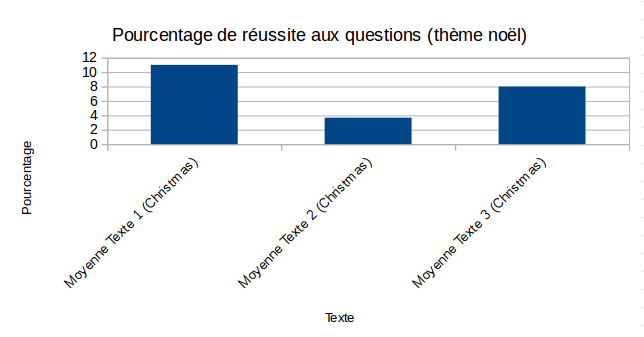
\includegraphics[scale=0.5]{../Images/resultatChristmas.png}
\caption{Graphique résumant les réponses aux questions sur le thème noël}
\end{center}

\end{figure}

\begin{figure}[!h]
\begin{center}

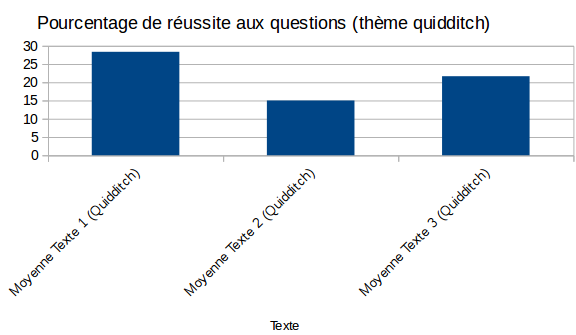
\includegraphics[scale=0.5]{../Images/resultatsQuidditch.png}
\caption{Graphique résumant les réponses aux questions sur le thème quidditch}
\end{center}

\end{figure}

\begin{figure}[!h]
\begin{center}

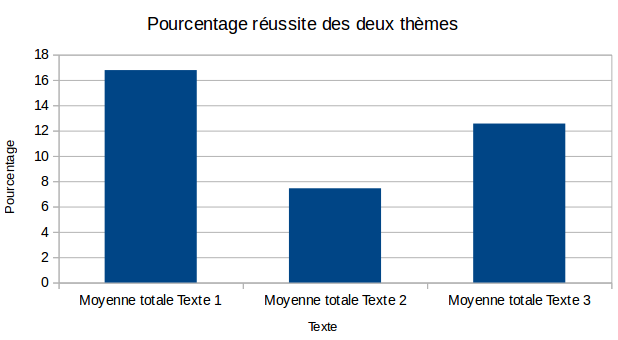
\includegraphics[scale=0.5]{../Images/ResultatsGlobal.png}
\caption{Graphique résumant les réponses aux questions (tout thème confondu)}
\end{center}



\end{figure}



\pagebreak

\begin{center}
\textbf{Conclusion générale}
\end{center}


Cette expérience a mis en avant le fait qu'une lecture automatisée au niveau des odeurs et des sons est surprenante mais agréable. Le lecteur n'a rien à faire à part lire et profiter du moment. Cependant, ce travail a mis en avant le côté trop divertissant de notre application. Choisir ses ambiances durant la lecture pourrait être une bonne chose, mais il faudrait bien le contrôler pour ne pas se perdre dedans et oublier la lecture en elle-même. Les sons doivent de plus être moins violent et avoir un fond moins répétitif tandis que les odeurs devraient rester peut-être plus longtemps en diffusion. Personne n'a compris le but du "mode manuel" : avoir un moyen de s'immerger dans la lecture par des sons que nous apprécions sans forcément qu'ils aient un lien avec la lecture.
Ce travail reste une réussite dans ce que nous avions à proposer : l'expérience avec des sons et odeurs automatiques a plu à tout le monde et permet de plus s'immerger et de mieux retenir le texte.









\begin{figure}[!h]
\begin{center}
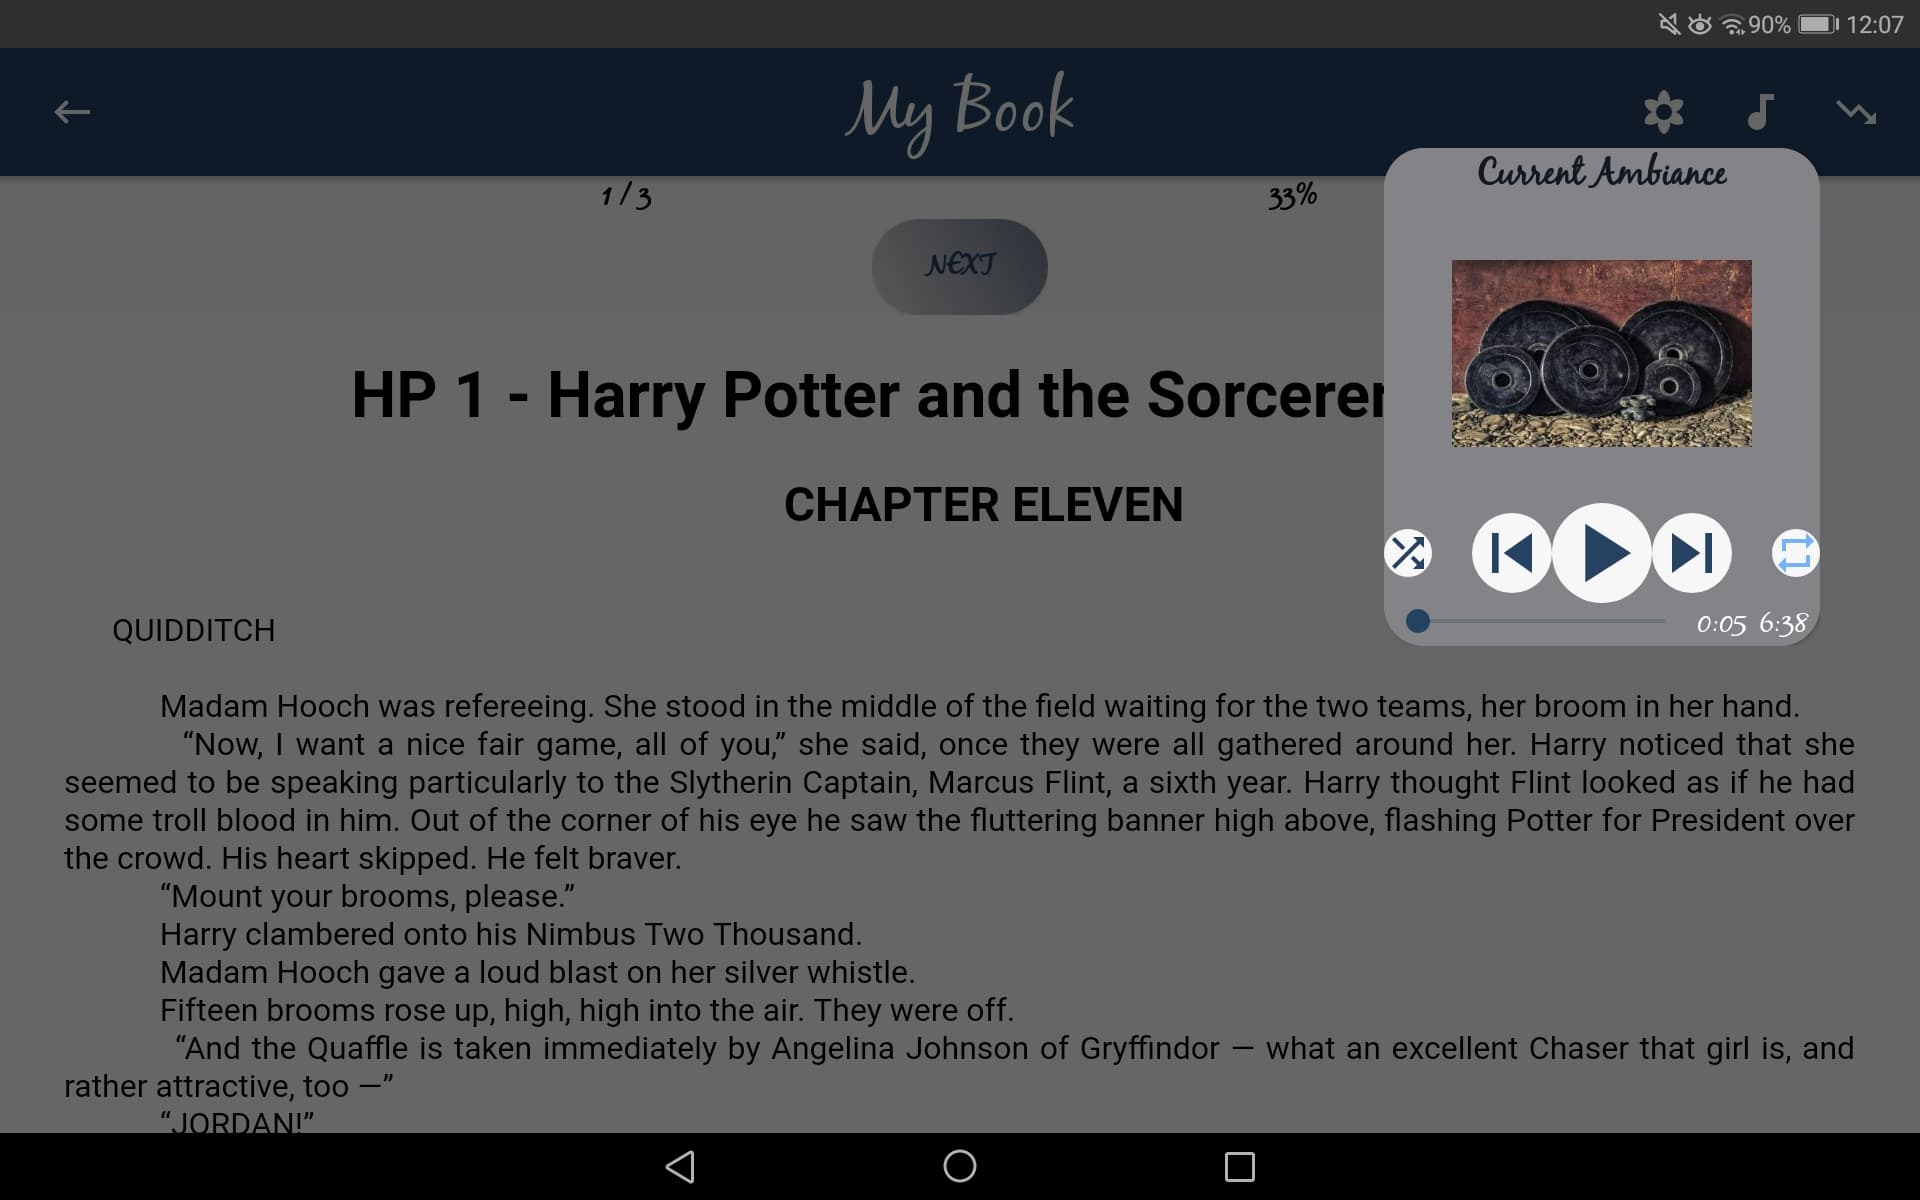
\includegraphics[scale=0.15]{../Images/texte1Ambiance.jpg}
\caption{Texte 1 (Quidditch) avec ambiance imposée}
\end{center}

\begin{center}

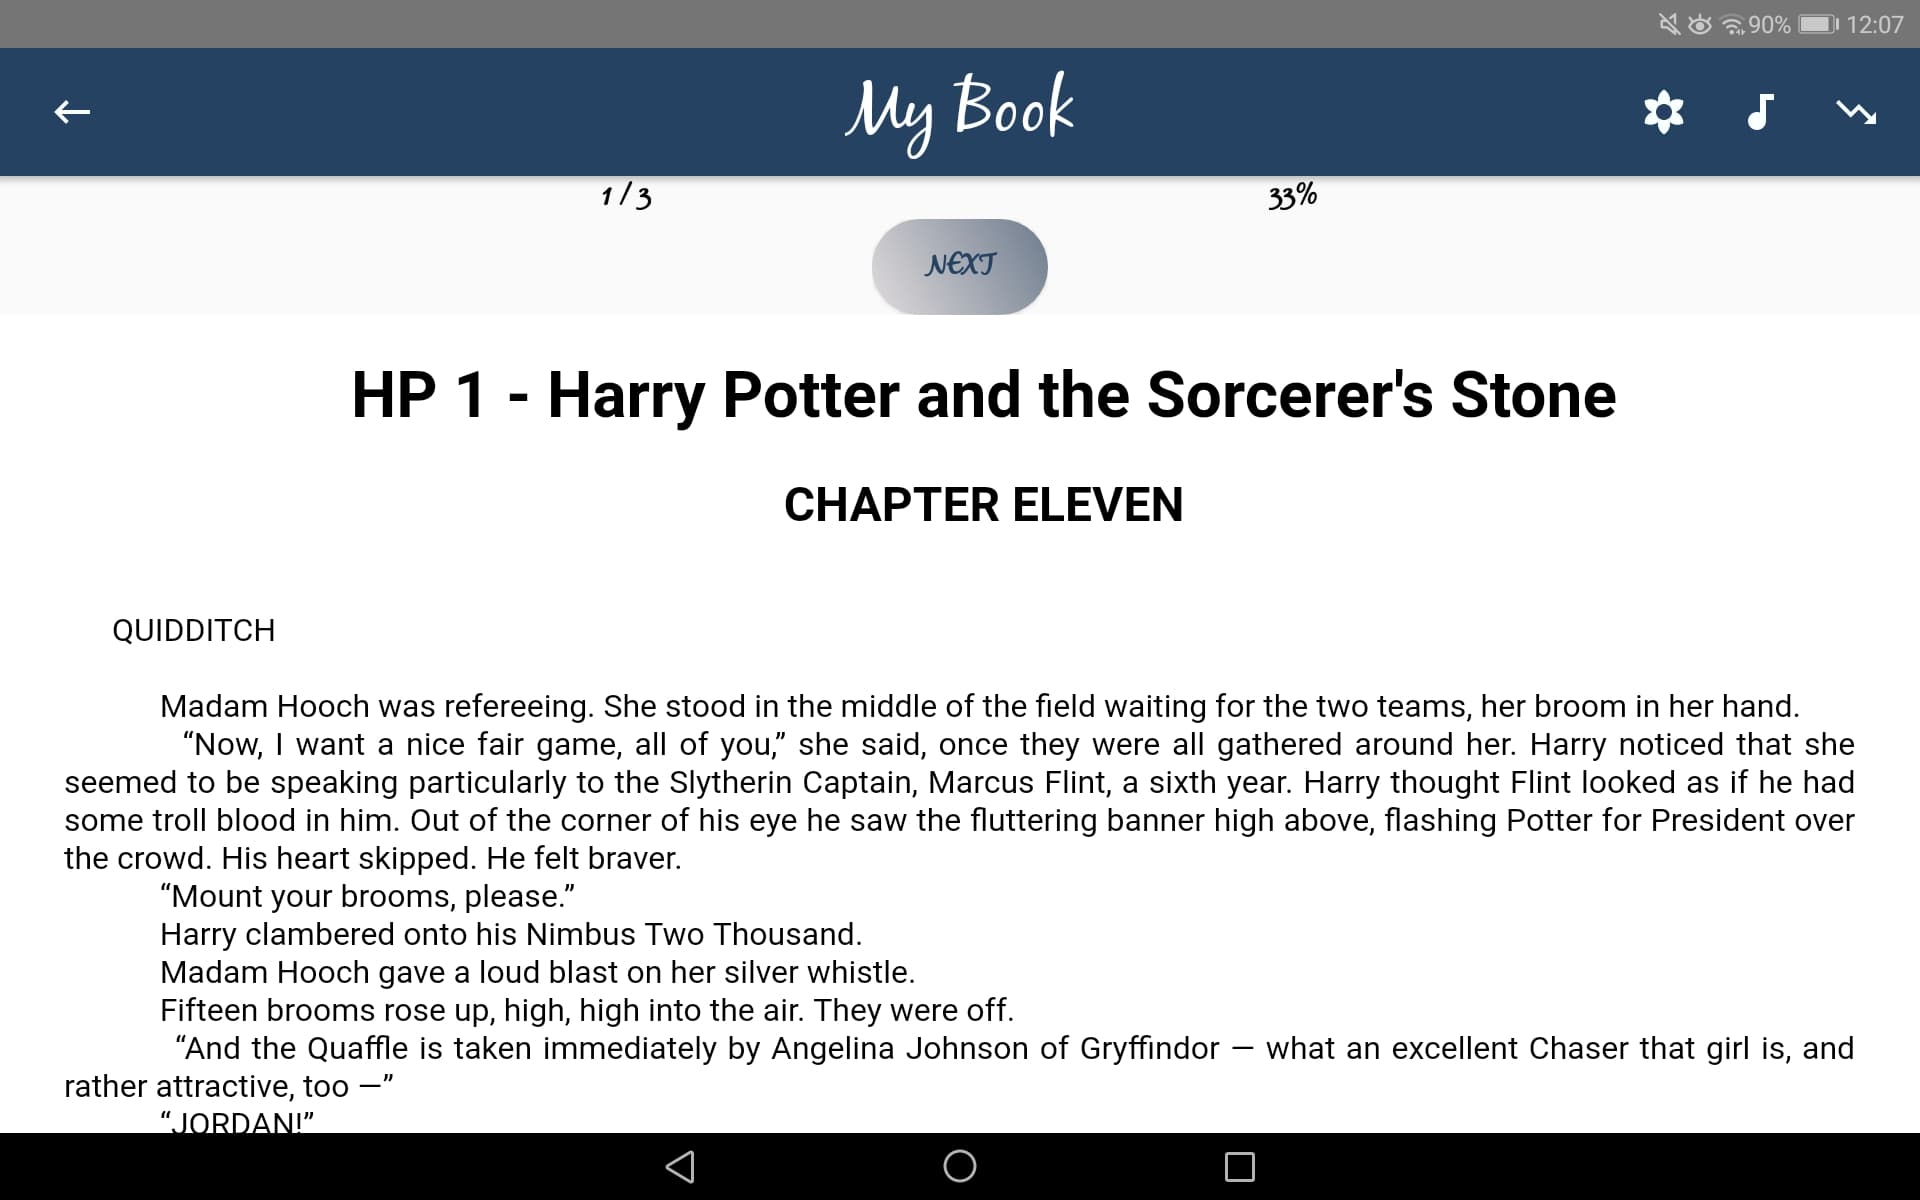
\includegraphics[scale=0.15]{../Images/texte1.jpg}
\caption{Texte 1 (Quidditch)  (sans pop-up ambiance) }

\end{center}

\begin{center}

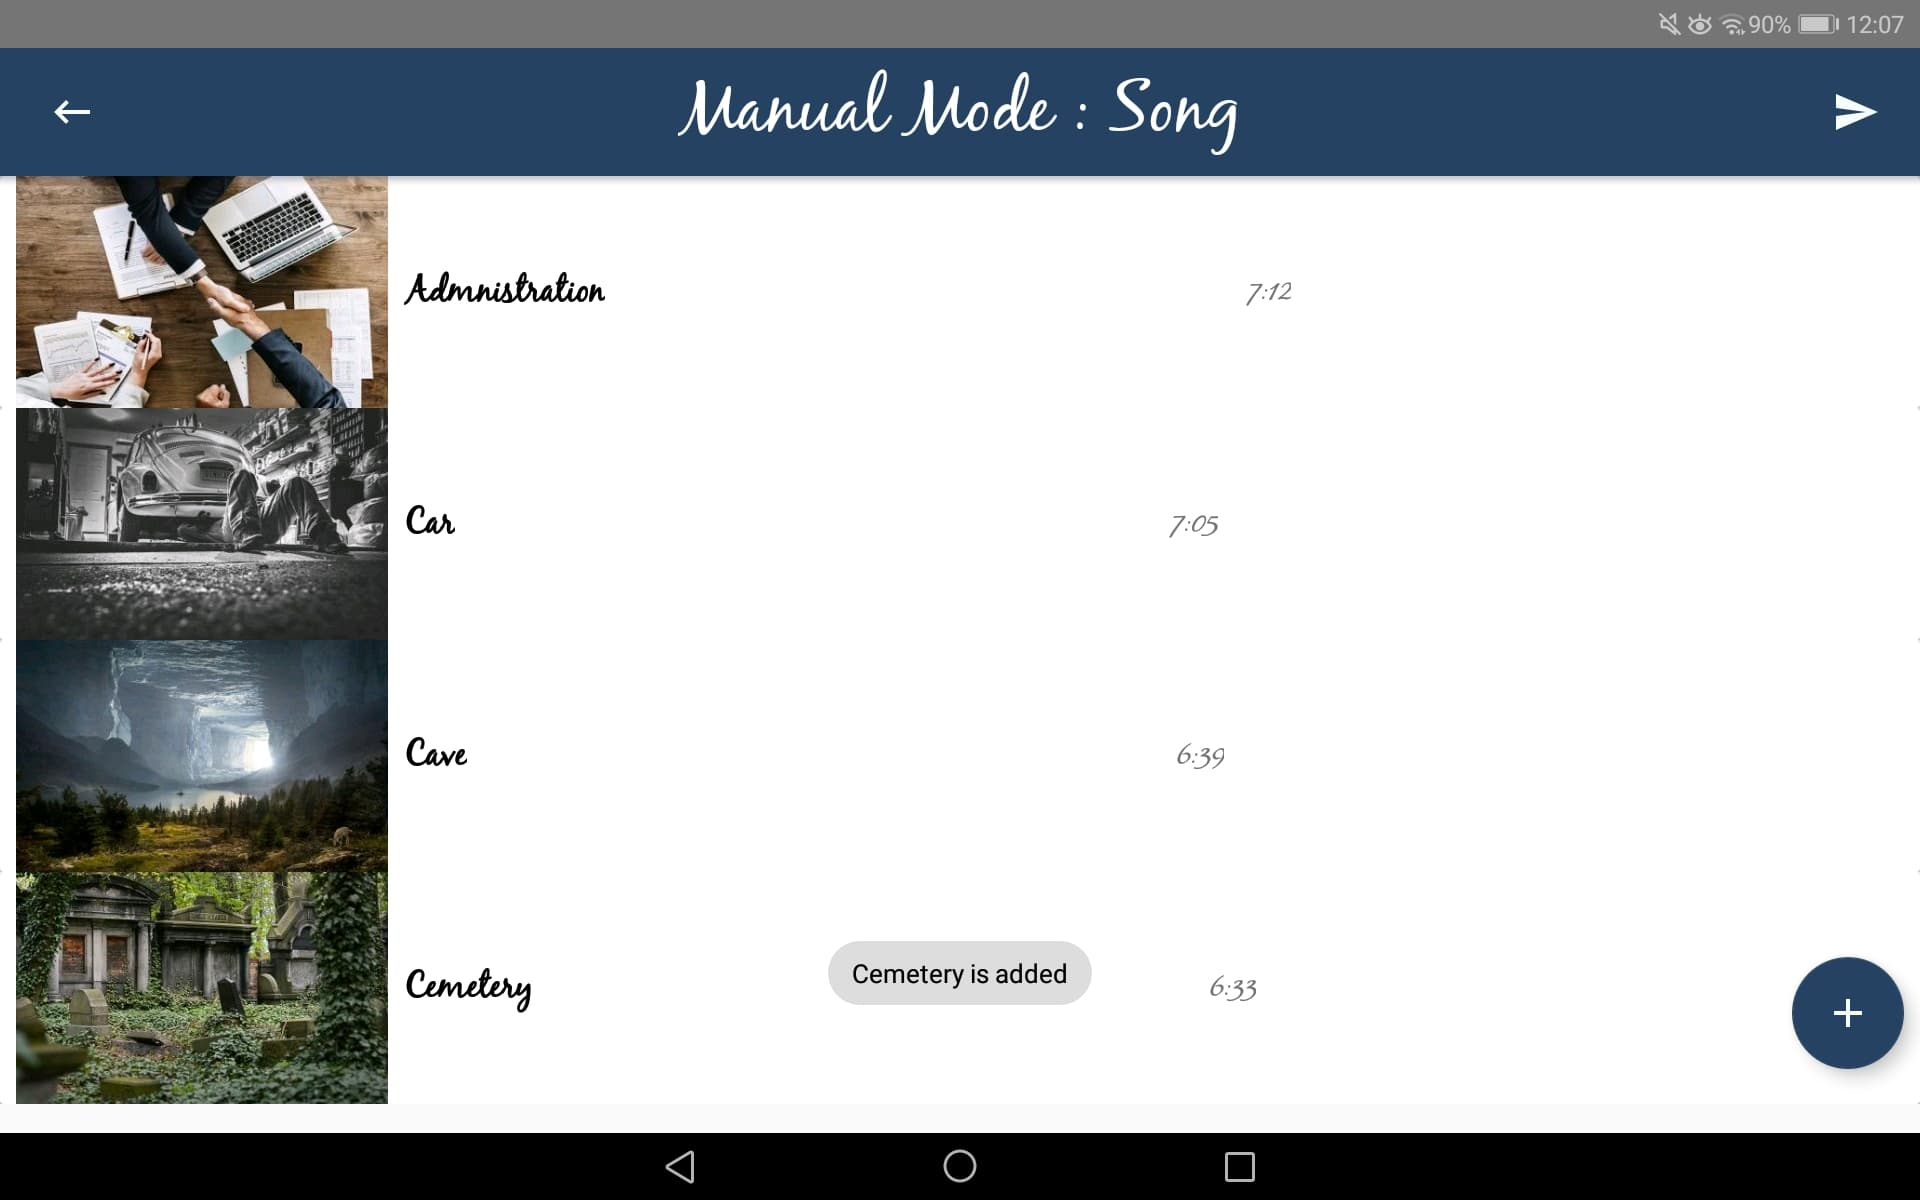
\includegraphics[scale=0.15]{../Images/selectAtmosphere.jpg}
\caption{Choix des ambiances (pour texte 2) }

\end{center}

\end{figure}


\begin{figure}[!h]
\begin{center}

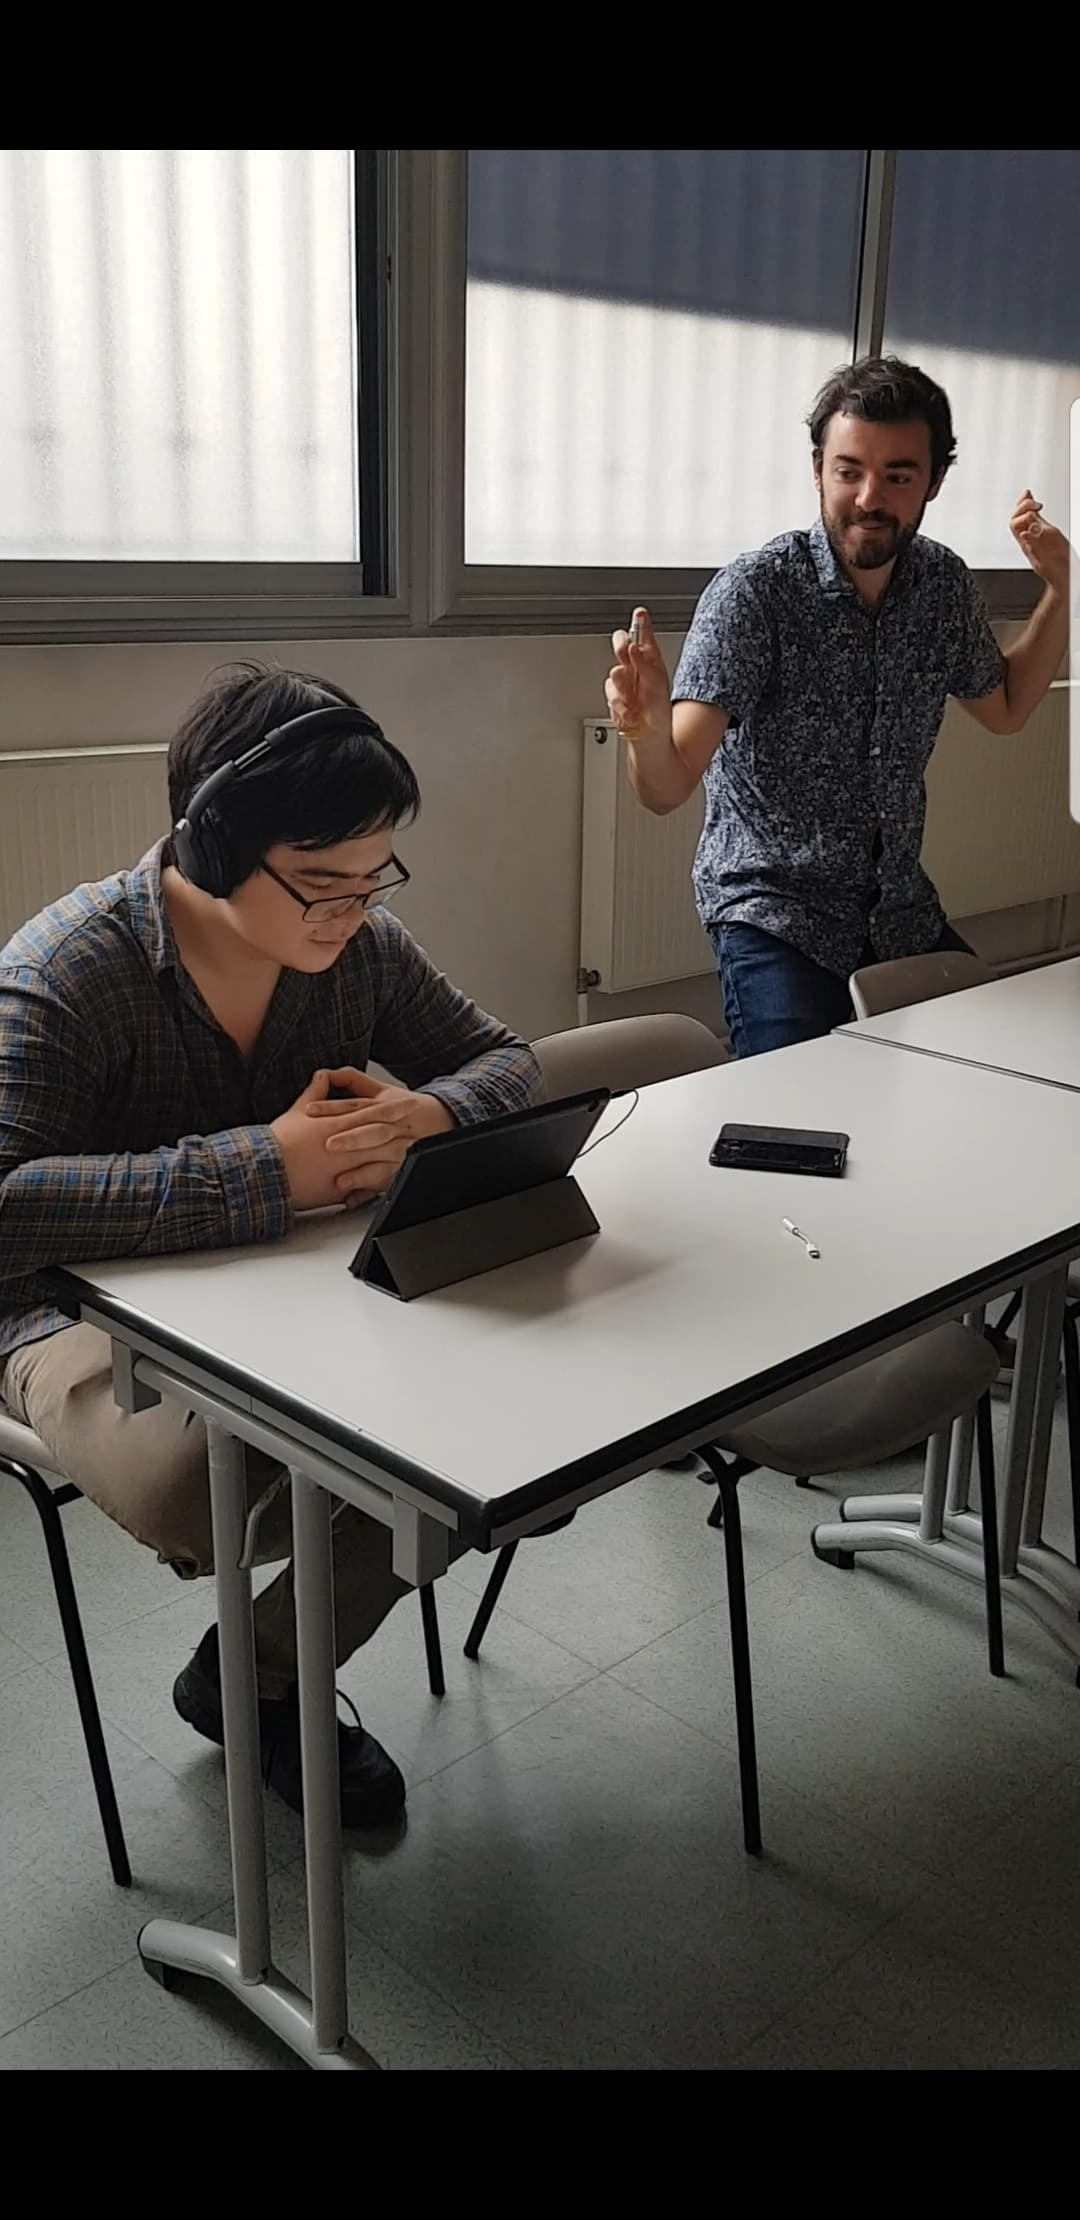
\includegraphics[scale=0.15]{../Images/odeurs.jpg}
\caption{Diffusion d'une odeur sur une personne interrogée }

\end{center}

\end{figure}




















\end{document}

